\chapter{Navržené řešení}
\label{sec:Propesed_solution}

Velká většina výzkumných prací, které se počítáním lidí v obraze zabývají, se snaží jejich množství určit na základě jediného snímku.
Toto je celkem logicky dáno jednodušší dostupností anotovaných datasetů, které jsou v případě, že se jedná pouze o jednotlivé snímky a ne videosekvence, mnohem obsáhlejší a zachycují větší množství nejrůznějších situací z rozličných úhlů pohledu.
Temporální informace ale mohou být při počítání objektů v obraze velmi cennou informací, kterou by neuronová síť mohla využít pro snazší řešení situací, kdy jsou lidé v obraze zakryti jinými lidmi či objekty, a zlepšit tak přesnost výsledného počtu.
Je totiž velmi nepravděpodobné, že člověk procházející zachycovanou scénou mezi dvěma po sobě jdoucími snímky zničehonic ze scény zmizí.
Je samozřejmě možné, že tento člověk například zašel za roh, nebo byl zakryt kolem projíždějící dodávkou, ale pokud je stále alespoň trochu patrné, že se v obraze nachází a je překryt pouze částečně, tak by měl být do výsledného počtu rozhodně započítán. Pokud by taková situace byla vyhodnocována pouze na základě jediného snímku, tak by nepochybně bylo přesné spočítání lidí obtížné i pro člověka. Předchozí snímky přitom často obsahují informace, které by při rozhodování, zda se opravdu jedná o člověka, mohly výrazně pomoci.

\begin{figure}[h!]
	\centering
	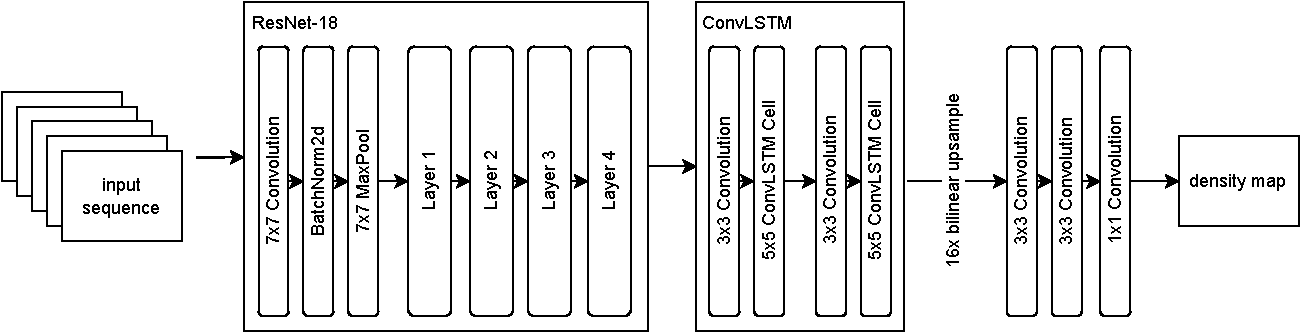
\includegraphics[width=\textwidth]{Figures/solution/net_structure.pdf}
	\caption{Struktura navržené sítě}
	\label{fig:proposed_net}
\end{figure}

Neuronová sít navržená v této práci se tohoto snaží využít a jejím cílem je vytvořit ze vstupní sekvence \(n\) po sobě jdoucích snímků dvoudimenzionální hustotní mapu, která vyobrazuje hustotu výskytu lidí v posledním snímku vstupní sekvence, a z ní estimovat množství lidí v něm. Na obrázku \ref{fig:proposed_net} je vyobrazena struktura sítě navržené v této práci.
Jak je z obrázku patrné, tak se skládá z několika částí, které budou v této kapitole blíže popsány.

\section{ResNet}
Residuální neuronová síť (ResNet) \cite{ResNet} byla poprvé představena v roce 2015, kdy vyhrála ImageNet Large Scale Visual Recognition Challenge, a svou architekturou silně ovlivnila budoucnost návrhu neuronových sítí.
Síla této neuronové sítě spočívá v tom, že přináší způsob, jak snížit vliv tzv. problému mizejícího gradientu (vanishing gradient problem).
Komplexita neuronových sítí se s každým rokem zvyšuje. Nejvíce se ale konvoluční neuronové sítě rozrůstají do hloubky. Čím je totiž neuronová síť hlubší, tím komplexnější příznaky dokáže extrahovat z původního vstupu a tím složitější funkce dokáže aproximovat.
Čím je ale neuronová síť hlubší, tím více se projevuje problém mizejícího gradientu.
Když je při trénování sítí šířena chyba pomocí algoritmu backpropagation, dochází k tomu, že její vliv je na svrchních vrstvách menší, než na hlubokých. Je-li tedy síť příliš hluboká, tak gradient je na svrchních vrstvách tak malý, že nedochází k přenastavení vah a tyto vrstvy se tedy nijak nemění.
Prohloubení sítě tedy v tomto případě ztrácí smysl a dokonce může mít negativní vliv na její výsledky.
Mělčí neuronové sítě proto mohou při řešení stejného problému dosáhnout mnohem lepších výsledků.

\begin{figure}[h!]
	\centering
	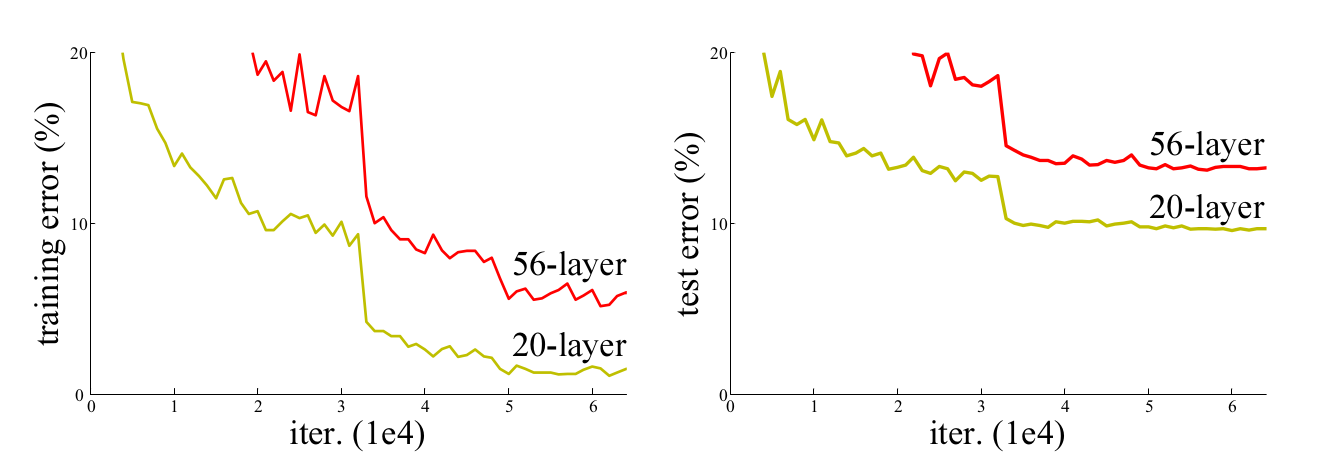
\includegraphics[width=0.7\textwidth]{Figures/solution/vanishing_gradient.png}
	\caption{Porovnání chyby při testování a trénování dvou sítí o hloubce 20 a 56 vrstev určených ke klasifikaci na datasetu CIFAR-10 \cite{ResNet}}
\end{figure}

Síť ResNet je tvořena reziduálními bloky, které jsou podobné VGG blokům \cite{VGG}.
Každý blok obsahuje dvě konvoluce o velikosti 3x3 a každá konvoluce je následovaná normalizací dávky (batch normalization) a aktivační funkcí ReLU.
Co ale reziduální blok přidává je tzv. zkratkové spojení (shortcut connection), které právě pomáhá snižovat vliv mizejícího gradientu.
Zkratkové spojení vezme vstupní hodnoty reziduálního bloku a přidá je k hodnotám před spuštěním druhé aktivační funkce.
V praxi to znamená, že vstupní hodnoty prochází v bloku dvěma cestami, kdy v jedné jsou změněny dvěma konvolucemi, zatímco v druhé se těmto konvolucím vyhnou. Při zpětném šíření chyby sítí se tedy chyba dostane do horních vrstev mnohem rychleji, takže navrhovaná síť může být mnohem hlubší.

\begin{figure}[h!]
	\centering
	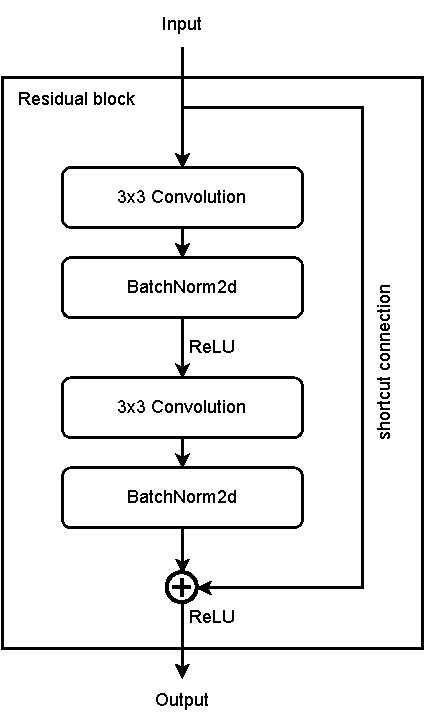
\includegraphics[width=0.3\textwidth]{Figures/solution/residual_block.pdf}
	\caption{struktura reziduálního bloku}
	\label{fig:residual_block}
\end{figure}

Síť ResNet je v navržené síti použita hned na vstupu a jejím cílem je zredukovat dimenzi vstupní sekvence po sobě jdoucích snímků a extrahovat z jednotlivých snímků důležité příznaky, které následně budou využity pro extrakci temporálních informací a konstrukci výsledné hustotní mapy.
Konkrétně je použita síť ResNet18, která obsahuje pouze čtyři reziduální bloky.
Tato varianta byla zvolena kvůli omezenému množství paměti na testovacím stroji.

\endinput
\section{ConvLSTM}
Tradiční konvoluční neuronové sítě jsou výborným nástrojem pro zjišťování a práci s příznaky v prostorové doméně. Pokud je ale potřeba kromě prostorových dat nutné pracovat i s temporálními informacemi, musíme použít jiný nástroj. V takovém případě se nabízí použití ConvLSTM (Convolutional Long Short-Term Memory) sítě. Ta byla poprvé představena v roce 2015 v článku \cite{ConvLSTM}. Pro pochopení, jak ConvLSTM funguje, je ale nejdříve důležité pochopit, na jakém principu funguje tradiční LSTM síť, na které je ConvLSTM založená.

LSTM patří do skupiny rekurentních neuronových sítí (RNN), které slouží ke zpracování sekvenčních dat, kde existuje závislost aktuálního vstupu na předchozím.
Problémem použití klasických neuronový sítí na taková data je, že neuronová síť řeší každý vstup zvlášť a nemá žádný mechanismus, pomocí kterého by si dokázala spojit předchozí vstupy s těmi aktuálními.
Samozřejmě by se nabízela možnost dát na vstup neuronové sítě celou vstupní sekvenci, nebo alespoň její část, která se nachází bezprostředně před aktuálním vstupem, avšak to by znamenalo, že výsledná neuronová síť by musela být mnohem komplexnější, což by znamenalo větší nároky na výpočetní sílu a velikost trénovací množiny.
Rekurentní neuronové sítě tento problém řeší tím, že přidávají stavové proměnné, které ukládají informace o předchozích vstupech a jsou zpracovávány společně s aktuálním vstupem.

\begin{figure}[h!]
	\centering
	\subfloat[Architektura RNN]{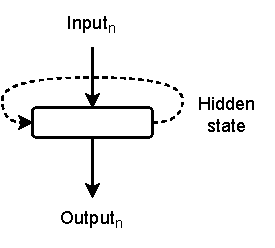
\includegraphics[width=0.3\textwidth]{Figures/solution/RNN_architecture.pdf}}
	\subfloat[Architektura RNN (rozvinutá)]{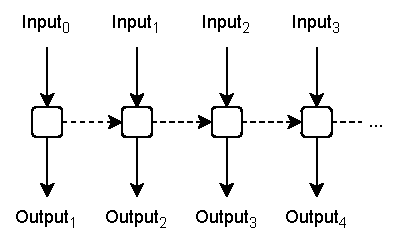
\includegraphics[width=0.4\textwidth]{Figures/solution/RNN_architecture_unrolled.pdf}}
	\caption{Diagram architektury RNN}
	\label{fig:RNN_architecture}
\end{figure}

Jak je patrné z obrázku \ref{fig:RNN_architecture}, tak pro každý vstup ve zpracovávané sekvenci je na základě tohoto vstupu a stavu stavové proměnné vzniklé zpracováním předchozího vstupu vytvořen výstup a nový stav skryté proměnné.
Jelikož je tato skrytá proměnná každým aktuálním vstupem měněna, dochází k tomu, že informace, která do ní byla zapsána při zpracování starších vstupů, ztrácí na významu a je překryta novějšími vstupy.
Rekurentní neuronové sítě z tohoto důvodu trpí problémy s dlouhodobější pamětí a jejich paměť je spíše krátkodobá.

LSTM se tento problém snaží vyřešit tak, že je specificky designovaná tak, aby více udržovala i dlouhodobější informace \cite{understaning_lstm}.
Samotný koncept LSTM již je celkem starý.
Poprvé byla síť LSTM představena v roce 1997 Hochreiterem a Schmidhuberem \cite{LSTM}.
Schéma LSTM je zobrazeno na obrázku \ref{fig:LSTM_architecture} a mnohým může připomínat strukturu logického obvodu.
Od toho se odvíjí i názvosloví, které tuto problematiku obklopuje, jelikož často mluví o branách.
Jak může být ze schématu patrné, tak LSTM má dvě stavové proměnné.

\begin{figure}[h!]
	\centering
	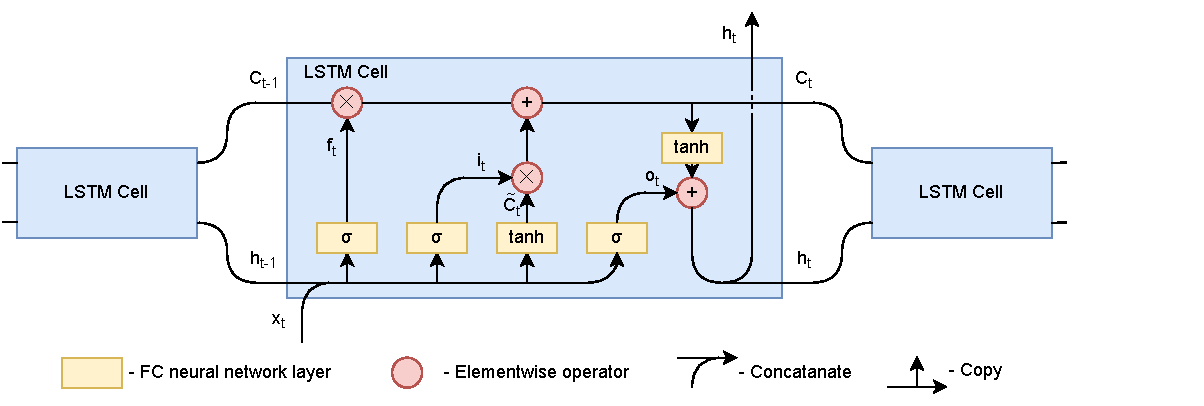
\includegraphics[width=\textwidth]{Figures/solution/LSTM_diagram.pdf}
	\caption{Struktura LSTM}
	\label{fig:LSTM_architecture}
\end{figure}



První z nich (procházející vrchní částí diagramu) slouží k ukládání dlouhodobých informací a často se nazývá stav buňky (cell state). Druhá z nich se nazývá skrytý stav (hidden state) a jedná se o paměť, se kterou LSTM buňka aktivně pracuje a na základě které rozhoduje, jak postupovat dále.
Postup vyhodnocování vstupních informací se dá rozdělit do několika kroků.
V následujících vzorcích v čase \(t\) vyjadřuje \(C_t\) stav buňky, \(h_t\) skrytý stav a výstup, \(x_t\) vstup a \(W_{...}\) a \(b_{...}\) značí váhy a zkreslení (bias) neuronů popisovaných bran.

\begin{enumerate}

\item Na základě informací, které jsou obsaženy ve skrytém stavu a vstupním vektoru, je rozhodnuto, jaké informace ze stavu buňky budou ponechány a jaké budou zapomenuty.
O toto se stará tzv. zapomínací brána (Forget gate), tvořená plně propojenou vrstvou se sigmoidální aktivační funkcí.
Tato brána je následována Hadamardovým součinem výsledku této operace se stavem buňky.

Má-li být informace uložená v daném prvku stavu buňky zapomenuta, nastaví plně propojená vrstva hodnotu v odpovídajícím prvku na nulu.
V případě, že má být informace v prvku ponechána tak, jak je, bude ve výsledku FC vrstvy jednička.
Výsledek FC vrstvy samozřejmě může být jakékoliv číslo v intervalu \(<0;1>\) v závislosti na tom, jak moc má být informace zapomenuta a její vliv na další výpočet snížen.
Tuto bránu lze vyjádřit rovnicí \ref{eq:forget_gate}. 

\begin{equation}
f_t = \sigma(W_f \cdot [h_{t-1}, x_t] + b_f)
\label{eq:forget_gate}
\end{equation}


\item Následuje rozhodnutí o tom, jaké nové informace mají být ve stavu buňky uloženy.
Podobně jako v předchozím kroce jsou vstupní data společně se skrytým stavem dána na vstup vstupní brány (Input gate) tvořené FC vrstvou se sigmoidální aktivační funkcí, která určuje, jaká data mají být zapamatována.

\begin{equation}
i_t = \sigma(W_i \cdot [h_{t-1}, x_t] + b_i)
\label{eq:input_gate}
\end{equation}

Než jsou ale data do stavu buňky přidána, jsou předtím zpracována vstupní modulační branou (Input Modulation gate), která je také tvořena FC vrstvou, ale používá jako aktivační funkci hyperbolický tangens (\(\tanh\)).
Výsledek této operace je po složkách vynásoben s výsledkem vstupní brány a tento násobek je opět po jednotlivých složkách přičten k patřičným složkám ve stavu buňky.

\begin{equation}
\widetilde{C}_t = \tanh(W_{\widetilde{C}} \cdot [h_{t-1}, x_t] + b_{\widetilde{C}})
\label{eq:input_modulation_gate}
\end{equation}

Tímto jsou ukončeny veškeré modifikace stavu buňky \(C_t\) které by se daly vyjádřit rovnicí \ref{eq:cell_state_modification}, kde operátor \(\circ\) značí Hadamardův součin.

\begin{equation}
C_t = f_t \circ C_{t-1} + i_t \circ \widetilde{C}_t
\label{eq:cell_state_modification}
\end{equation}


\item Zbývá ještě poslední krok, a tím je vytvoření skrytého stavu buňky, který je zároveň i jejím výstupem.
Ten je vytvořen ze stavu buňky, avšak předtím, než jsou data dána na výstup jsou modifikována FC vrstvou s aktivační funkcí \(\tanh\).
Následně je ještě rozhodnuto, jaká data jsou na výstup propuštěna a v jaké míře.
K tomuto účelu slouží výstupní brána (Output gate), která je opět tvořena FC vrstvou se sigmoidální aktivační funkcí.
Na vstupu tato brána bere vstupní data společně se skrytým stavem a na jejich základě rozhodne o tom, jaké informace ze stavu buňky budou propuštěny dále.

\begin{equation}
o_t = \sigma(W_o \cdot [h_{t-1}, x_t] + b_o)
\label{eq:output_gate}
\end{equation}

Výpočet výstupu LSTM buňky a jejího skrytého stavu lze tedy vyjádřit rovnicí \ref{eq:output}.

\begin{equation}
h_t = o_t \circ \tanh(C_t)
\label{eq:output}
\end{equation}

\end{enumerate}

V literatuře se dá narazit i na verzi LSTM, která využívá tzv. špehýrková spojení (peephole connections), která byla přidána do LSTM architektury Gersem a Schidhuberem v roce 2000. \cite{PeepLSTM}
Tato spojení způsobují, že ke vstupu všech bran, které mají sigmoidální aktivační funkci, je přidán i stav buňky. U zapomínácí a vstupní brány jde o \(h_{t-1}\), neboli stav buňky před jakýmikoliv modifikacemi, zatímco u brány výstupní je použit již modifikovaný stav  \(h_{t}\).
Brány tedy rozhodují nejen na základě aktuálního vstupu a skrytého stavu buňky, ale i podle obsahu stavu buňky.
Vzorce \ref{eq:forget_gate} a \ref{eq:input_gate} by tedy šly v tomto případě napsat podle vzoru \( A_t = \sigma(W_A \cdot [h_{t-1}, x_t, C_{t-1}] + b_A) \), kde za \(A\) dosadíme \(f\) nebo \(i\), a vzorec \ref{eq:output_gate} by vypadal \( o_t = \sigma(W_o \cdot [h_{t-1}, x_t, C_{t}] + b_o) \).


Konvoluční LSTM vrstvy ConvLSTM spojují výhody konvolučních vrstev, které jsou skvělé pro zpracování prostorových informací a LSTM vrstev, které dobře zpracovávají temporální informace, a proto jsou jedním z nástrojů, které je možné použít pro práci s časoprostorovými daty.

Na rozdíl od klasické LSTM vrstvy rozhoduje ConvLSTM o novém stavu buňky nejen na základě jejího vstupu a jejích skrytých stav a také na základě vstupů a skrytých stavů jejích sousedů.
Vstupy, výstupy a skryté stavy jsou z tohoto důvodu u ConvLSTM reprezentovány pomocí 3D tenzorů, jejichž poslední dvě dimenze jsou dimenze prostorové.
Na tyto tenzor jsou následně použity konvoluční operace pro výpočet nového stavu buňky a skrytého stavu. Ekvivalenty vzorců popisujících jednotlivé brány v LSTM tedy vypadají následovně.

\begin{equation}
f_t = \sigma(W_{f} * [x_t, h_{t-1}] + b_f)
\label{eq:ConvLSTM_forget_gate}
\end{equation}

\begin{equation}
i_t = \sigma(W_{i} * [x_t, h_{t-1}] + b_i)
\label{eq:ConvLSTM_input_gate}
\end{equation}

\begin{equation}
\widetilde{C}_t = \tanh(W_{c} * x_t + b_c)
\label{eq:ConvLSTM_input_modulation_gate}
\end{equation}

\begin{equation}
o_t = \sigma(W_{o} * [x_t, h_{t-1}] + b_o)
\label{eq:ConvLSTM_output_gate}
\end{equation}

I u ConvLSTM je možné se setkat s verzí obsahující špehýrková spojení.
V tomto případě ale není stav buňky pouze konkatenován se vstupem a skrytým stavem před tím, než je na ně použita konvoluce.
Místo toho je k nim přidán až po provedení této operace a místo konvoluce je svými vahami upraven pouze Hadamardovým součinem.

Aby šel vstup, stav buňky a skrytý stav jednoduše konkatenovat, musí mít stejné prostorové rozměry.
Z tohoto důvodu musí být velikost obrázků, které bude síť zpracovávat, známa předem, jelikož skryté stavy ConvLSTM buňky musí být inicializovány na správnou velikost.

Změnou velikosti konvoluční masky se dá měnit na jak rychle pohybující se objekty bude výsledná síť citlivá.
Je jasné, že maska o velikosti 3x3 nebude efektivní pro zpracování objektu, který překoná během jediného snímku polovinu celého scény, která má na snímku stovky pixelů.
Lidé se však moc rychle nepohybují a v případě, kdy jsou snímání kamerou se snímací frekvencí 30Hz, je tento pohyb o to menší. Síť ResNet, která je použita bezprostředně před ConvLSTM vrstvami navíc zmenšuje prostorové dimenze vstupních vektorů, tudíž v tomto případě je maska o velikosti 3x3 dostatečná.
V navržené síti jsou proto použity 2 po sobě jdoucí ConvLSTM vrstvy s velikostí konvoluce 3x3, které následují po extrakci prostorových příznaků pomocí sítě ResNet.
Dvě vrstvy jsou použity z toho důvodu, že v případě, že je v síti použito více ConvLSTM vrtstev, je taková síť schopná ze vstupní sekvence extrahovat složitější časoprostorové příznaky.

\endinput
\section{Účelová funkce}

Cílem zbytku navržené neuronové sítě je z časoprostorových příznaků získaných v předchozích částech vytvořit výslednou hustotní mapu.
Specificky má síť za úkol vytvořit hustotní mapu, která odpovídá "základní pravdě" (Ground Truth), posledního snímku právě zpracovávané sekvence vstupních snímků.
Jednou z možností by bylo učit síť co nejblíže replikovat hustotní mapy tvořené Gaussiány vloženými do hustotní mapy v bodech, kde se v posledním snímku nacházejí jednotlivé lidské hlavy, jak bylo popsáno v kapitole \ref{sec:History}.
V takovémto případě je často použita účelová funkce, které je definovaná na základě sumy chyby v jednotlivých bodech výsledného obrazu. Příkladem by mohla být například střední kvadratická chyba \ref{eq:MSE_loss}, nebo nebo absolutní chyba \ref{eq:AE_loss}.

\begin{equation}
loss_{MSE} = \frac{1}{n} \sum_{i=1}^{n} (x_i - y_i)^2
\label{eq:MSE_loss}
\end{equation}

\begin{equation}
loss_{AE} = \frac{1}{n} \sum_{i=1}^{n} |x_i - y_i|
\label{eq:AE_loss}
\end{equation}

Dle \cite{Bayesian_Crowd_Counting, DM_Count} ale není využití těchto účelových funkcí závislých na jednotlivých pixelech optimální, jelikož výsledná přesnost natrénované neuronové sítě je silně závislá na kvalitě vygenerovaných hustotních map základní pravdy.
Získání vysoce kvalitní základní pravdy je ale obtížné.
Datasety používané pro trénování neuronových sítí jsou totiž velmi obsáhlé a manuální anotace jednotlivých snímků, kde musí být označena každá hlava, je proto časově velmi náročná.
Anotace se z toho důvodu u mnoha významných datasetů omezuje pouze na pozice hlav a nijak nebere v potaz jejich velikost v obraze. U Gaussiánů je proto často použit konstantní parametr rozptylu a vliv perspektivy způsobující rozdílné velikosti hlav v obraze není nijak brán v úvahu.
Kvůli částečným zakrytím, ke kterým může v obraze docházet, může být problémem také přesné určení pozice hlavy.
Jednotliví lidé anotující datasety také mohou mít jiné preference k tomu, kam bod označující hlavu umisťují. V některých případech to může například být doprostřed čela, jindy ale třeba na nos.
Tyto faktory znamenají, že vygenerovaná hustotní mapa často není optimální, což může vést ke zhoršení přesnosti trénované sítě.

Z tohoto důvodu byla v navržené síti použita účelová funkce navržená ve článku Distribution Matching for Crowd Counting \cite{DM_Count}.
Metoda navržená v tomto článku se na problém počítání objektů v obraze dívá jako na problém párování distribučních funkcí (Distribution Matching) a jejím výstupem je hustotní mapa, pro kterou platí, že suma jejích jednotlivých bodů se rovná počtu lidí v obraze, stejně jako u metody vkládající do mapy Gaussiány. Narozdíl od této metody ale Gaussiány nepotřebuje.

Tato účelová funkce se skládá ze tří částí.
Tyto tři části jsou menšími účelovými funkcemi, které jsou ve výsledné funkci spojeny dohromady pomocí lineární kombinace.
První z nich autoři nazývají "Counting Loss".
Ta je definovaná vzorcem \ref{eq:counting_loss}.
Základní pravda je v následujících vzorcích vyjádřena písmenem \(z\), které reprezentuje binární mapu pozic jednotlivých hlav v obraze, zatímco \(\hat{z}\) reprezentuje predikovanou hustotní mapu.
\(\|z\|_1\) a \(\|\hat{z}\|_1\) jsou L1 normami vektorizovaných matic \(z\) a \(\hat{z}\) a vyjadřují počet lidí v základní pravdě a v predikované hustotní mapě.
Counting loss je vyjádřena jako absolutní hodnota rozdílu těchto počtů a jejím cílem je při hledání optima konečné účelové funkce zajistit, aby se predikovaný počet co nejvíce blížil opravdovému počtu lidí v obraze.

\begin{equation}
loss_C(z, \hat{z}) = \Big|\|{z}\|_1 - \|\hat{z}\|_1\Big|
\label{eq:counting_loss}
\end{equation}

Druhou částí účelové funkce je tzv. "Optimal Transport Loss". 
Tato funkce využívá metod z matematické oblasti dopravních problémů.
Jedním z prvních matematiků, který se touto oblastí zabýval byl Gaspard Monge, vévoda z Péluse, který se v roce 1781 zabýval problematikou konstrukce vojenského opevnění a způsoby, jak tvorbu takové stavby zefektivnit.
Přesněji se zaměřil na konstrukci příkopů a valů.
Je logické, že při konstrukci valu chceme využít zeminu, která byla vykopána z příkopu.
Všechna tato zemina ale musí být přesunuta, a z ekonomických důvodů chceme, aby k přesunu došlo co nejoptimálnějším způsobem.
Práce vynaložená na přesun zeminy z příkopu na val tedy musí být co nejnižší.

\begin{figure}[h!]
	\centering
	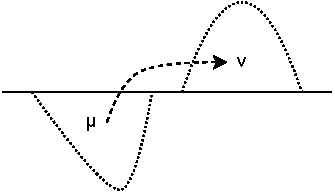
\includegraphics[width=0.5\textwidth]{Figures/solution/Optimal_transport.pdf}
	\caption{Ukázka problému optimálního přesunu}
	\label{fig:RNN_architecture}
\end{figure}


Příkop, ze kterého je zemina brána je označen písmenem \(\mu\) a val, na který je vršena písmenem \(\nu\).
Je jasné, že hmota při přemisťování nemůže vznikat ani zanikat, takže objem hmoty navršené na val musí být roven objemu hmoty vykopané z příkopu. 
Rozložení \(\mu\) a \(\nu\) tedy můžeme vyjádřit jako pravděpodobnostní míry na prostorech \(X\) a \(Y\).
Dále můžeme definovat funkci ceny \(c : X \times Y  \rightarrow \R^+ \), která vyjadřuje práci nutnou k přemístění jedné jednotky hmoty z bodu \(x \in X\) do bodu \(y \in Y\).
Mongeho-Kantorovichův problém optimálního přesunu (Optimal Transport) se zabývá tím, jak přesunout všechnu hmotu z \(\mu\) do \(\nu\) tak, aby celková cena přesunu \(c\) byla minimální.

V \cite{DM_Count} definují optimální přesun pomocí vzorce \ref{eq:ot_1}, kde \(C\) značí matici obsahující všechny ceny přemístění hmoty z bodů v \(\mu\)  do bodů v \(\nu\) a \(\Gamma\) je množinou všech možných způsobů, jak tyto body přemístit.

\begin{equation}
\mathcal{W}(\mu, \nu) = \min_{\gamma in \Gamma} \langle C, \gamma \rangle
\label{eq:ot_1}
\end{equation}

Tato minimální cena může být použita jako metrika pro porovnání podobnosti dvou měr pravděpodobnosti.
Lze na to nahlížet tak, že čím méně zeminy musí být přemístěno z hromady \(\mu\), abychom dostali hromadu \(\nu\), tím podobnější si \(\mu\) a \(\nu\) musí být.
Optimal Transport Loss přesně tohoto principu využívá pro porovnání výsledné predikce sítě a 
základní pravdy.
Aby se tyto mapy daly pomocí Mongeho-Kantorovichova optimálního přesunu porovnat, jsou před výpočtem metriky znormalizovány, aby suma přes každou z nich byla rovna jedné.
Jako cenovou funkci použili autoři \cite{DM_Count} kvadrát Euklidovské vzdálenosti bodů v planární mapě \(c(z(i), \hat{z}(j)) = \|z(i) - \hat{z}(j)\|_2^2\), kde \(z(i)\) a \(\hat{z}(j)\) jsou koordináty bodů \(i\) a \(j\).

\begin{equation}
loss_{OT}(z, \hat{z}) = \mathcal{W}\bigg(\frac{z}{\|z\|_1}, \frac{\hat{z}}{\|\hat{z}\|_1}\bigg) 
\label{eq:ot_loss}
\end{equation}

Pro získání gradientu, který může být sítí zpětně šířen a na jehož základě dojde k přenastavení jejích vah, použili autoři duální problém k optimálnímu přesunu, jenž byl formulován Leonidem Kantorovičem.
Caffarelli \cite{Caffarelli_dual_problem} tento problém připodobňuje k situaci, kdy je pro přemístění zeminy z \(\mu\) do \(\nu\) použit externí přepravce, který si v nechává platit v bodě naložení \(\mu(x_i)\) a v bodě vyložení \(\nu(y_i)\).
Jeho ceny nesmí být vyšší, než cena \(c(x_i, y_i)\), jelikož by to bylo pro objednatele přepravy nevýhodné a přepravce by si proto neobjednal.
Přepravce proto řeší, jak nastavit ceny, aby maximalizoval svůj zisk, avšak jeho cena nebyla vyšší, než cena, kterou by platil objednavatel, kdyby převoz zeminy organizoval sám.
Touto maximalizací musí nutně dojít ke stejné celkové ceně, jako je řešení rovnice \ref{eq:ot_1}.
V \cite{DM_Count} je tento problém formulován rovnicí \ref{eq:ot_2}, kde \(\alpha\) a \(\beta\) jsou výplatní funkce, udávající, kolik si přepravce účtuje za naložení a vyložení materiálu.

\begin{equation}
\mathcal{W}(\mu, \nu) = \max_{\alpha, \beta \in \R^n} \langle \alpha, \mu \rangle + \langle \beta, \nu \rangle; \alpha_i + \beta_j  \leq c(x_i, y_j),  \forall i, j
\label{eq:ot_2}
\end{equation}

Rovnice \ref{eq:ot_loss} lze s použitím duálního problému přepsat jako \( loss_{OT}(z, \hat{z}) = \bigg \langle \alpha^*, \frac{z}{\|z\|_1} \bigg \rangle + \bigg \langle \beta^*, \frac{\hat{z}}{\|\hat{z}\|_1} \bigg \rangle \), kde  \(\alpha^*\) a \(\beta^*\) jsou řešeními \ref{eq:ot_2}, z čehož se dá vypočítat gradient.

\begin{equation}
\frac{\partial loss_{OT}}{\partial \hat{z}} = \frac{\beta^*}{\|\hat{z}\|_1} - \frac{ \langle \beta^*, \hat{z} \rangle}{\|\hat{z}\|_1^2}
\label{eq:ot_2}
\end{equation}

Pro zjištění řešení \(\alpha^*\) a \(\beta^*\) používají autoři Sinkhornův algoritmus.
Při jeho použití síť z počátku rychle konverguje do lokálního optima, avšak tato konvergence se také rychle zpomaluje.
Jelikož autoři omezili množství iterací Sinkhornova algoritmu, vrací tento algoritmus pouze přibližná řešení \(\alpha^*\) a \(\beta^*\), což způsobuje, že predikovaná hustotní mapa bude  podobná základní pravdě, ale nebude identická.
Toto podle autorů ve výsledné hustotní mapě způsobuje problémy, které nastávají hlavně v těch částech scény, kde je hustota lidí nízká a lidé jsou separováni.

Pro zpřesnění predikcí neuronové sítě v těchto problematických případech zavedli autoři do výsledné účelové funkce třetí část a to tzv. "Total Variation Loss".
Celková variační vzdálenost může být stejně jako cena optimálního přesunu použita pro porovnání dvou pravděpodobnostních měr \(\mu\) a \(\nu\) na stejném měřitelném prostoru \(\mathcal{A}, \mathcal{F}\) \cite{Total_variation}.
Vzdálenost těchto dvou pravděpodobnostních měr je definovaná následujícím vzorcem. (V literatuře se vyskytuje i verze, kdy je tato vzdálenost definovaná, jako dvojnásobek uvedeného vzorce, čímž se dá zbavit \(\frac{1}{2}\).)

\begin{equation}
\delta_{TV}(\mu, \nu) = \sup_{\mathcal{A} \in \mathcal{F}} (\mu(\mathcal{A}) - \nu(\mathcal{A})) = \frac{1}{2}\|\mu - \nu\|_1
\label{eq:total_variation}
\end{equation}

Budou-li \(\mu\) a \(\nu\) zcela disjunktní a nebudou tedy sdílet žádnou "hmotu", bude hodnota takto definované metriky rovna jedné.
Čím více "hmoty" sdílí, tím menší tato hodnota bude.
Při minimalizaci tedy dochází k tomu, že se \(\mu\) a \(\nu\) mnohem více překrývají a jsou-li identické, je hodnota \(\delta_{TV}(\mu, \nu)\) rovna nule.

\begin{equation}
loss_{TV}(z, \hat{z}) = \delta_{TV} \bigg( \frac{z}{\|z\|_1}, \frac{\hat{z}}{\|\hat{z}\|_1} \bigg)
= \frac{1}{2} \bigg\| \frac{z}{\|z\|_1} - \frac{\hat{z}}{\|\hat{z}\|_1} \bigg\|_1
\label{eq:tv_loss}
\end{equation}


Výsledná účelová funkce je, jak již bylo dříve zmíněno, lineární kombinací funkcí "Counting Loss",  "Optimal Transport Loss" a "Total Variation Loss". Parametry \(\lambda_1\) a \(\lambda_2\) slouží k nastavení síly vlivu "Optimal Transport Loss" a "Total Variation Loss" ve výsledné účelové funkci.
Aby autoři zajistili, že "Total Variation Loss" a "Optimal Transport Loss" budou mít stejné měřítko, je výsledek "Total Variation Loss" vynásoben počtem lidí v základní pravdě.

\begin{equation}
loss(z, \hat{z}) = loss_{C}(z, \hat{z}) + \lambda_1 loss_{OT}(z, \hat{z}) + \lambda_2 \|z\|_1 loss_{TV}(z, \hat{z})
\label{eq:overall_loss}
\end{equation}



\endinput

\endinput